\documentclass[conference]{IEEEtran}
\IEEEoverridecommandlockouts
\usepackage{amsmath,amssymb,amsfonts}
\usepackage{algorithmic}
\usepackage{graphicx}
\usepackage{textcomp}
\usepackage{xcolor}
\usepackage{float}
\usepackage[sorting=none, style=nature]{biblatex}
\addbibresource{ref.bib}
\usepackage[hidelinks]{hyperref}


\def\BibTeX{{\rm B\kern-.05em{\sc i\kern-.025em b}\kern-.08em
T\kern-.1667em\lower.7ex\hbox{E}\kern-.125emX}}
\begin{document}

    \title{Public Ledger for Auctions}

    \author{\IEEEauthorblockN{Cláudia da Costa Maia}
    \IEEEauthorblockA{up201905492@fc.up.pt}
    \and
    \IEEEauthorblockN{Fabiana Manuela Alves}
    \IEEEauthorblockA{up201404791@fc.up.pt }
    \and
    \IEEEauthorblockN{Junior Monteiro}
    \IEEEauthorblockA{up202209374@fc.up.pt}
    }

    \maketitle
    \begin{abstract}
        Este projeto tem como objetivo criar uma rede Kademlia com blockchain para uma aplicação de leilões descentralizada e segura. A rede Kademlia será responsável por gerenciar participantes e itens do leilão, enquanto a blockchain armazenará todas as ofertas e transações realizadas. A implementação inclui conceitos de P2P e DHT, mecanismos de criptografia e autenticação. O algoritmo de Proof-of-Work é utilizado para validar as transações e adicionar novos blocos à cadeia.

    \end{abstract}


    \begin{IEEEkeywords}
        Secure P2P; Kademlia DHT; Sybil and Eclipse attacks; Auction mechanisms; Distributed ledger; proof-of-work; proof-of-stake.........
    \end{IEEEkeywords}


    \section{Introdução}
    Este relatório descreve a implementação de uma rede Kademlia com blockchain para aplicação de leilões. O objetivo deste projeto é criar uma plataforma descentralizada e segura para a realização de leilões, onde a rede Kademlia gerencia os participantes e os itens do leilão, enquanto a blockchain armazena as ofertas e transações. O projeto foi dividido em três partes: (1) sobreposição P2P segura, (2) registro distribuído e seguro e (3) mecanismos de leilão.\\


    \section{Sobreposição P2P segura (\textit{Secure P2P overlay})}

    A sobreposição P2P é baseada em Kademlia DHT e é responsável por gerenciar os nós participantes da rede. A abordagem utilizada é sem permissão, o que significa que os nós não precisam ser conhecidos "a priori". Para garantir a segurança da rede, são implementados mecanismos de confiança e de comunicação gossip.

    \subsection{Kademlia DHT}
    O protocolo Kademlia é um sistema de tabela de hash distribuída (DHT) usado para localizar nós na rede P2P e armazenar informações de forma descentralizada.

    O Kademlia é baseado em uma chave de 160 bits, que é usada para identificar cada nó na rede e usa a distância XOR para medir a proximidade entre os nós e organizar a rede em um espaço métrico.

    Os nós mantêm informações sobre os outros nós em uma tabela, \textit{Routing table}, dividida em \textit{k-buckets} de acordo com a proximidade das chaves. Cada \textit{k-bucket} contém informações sobre até k nós mais próximos a uma determinada chave. Estas informações sobre os respetivos nó são: \textit{IP address, port e NodeID}.
    Assim, se a tabela de roteamento de um nó já tiver o número máximo de nós em um determinado \textit{k-bucket}, ele removerá o nó mais antigo nesse \textit{k-bucket} para libertar espaço para o novo nó.
    Para além disso, cada nó contém: \textit{IP address, Port, Unique ID, Routing table e Storage}.

    Dentro da rede existe nós comuns, que fazem parte da rede e são responsáveis por armazenar e encaminhar os dados. E, nós \textit{bootstrap}, de inicialização, que conhecem todos os outros nós e são os nós responsáveis por ajudar os novos nós a ingressarem na rede. Esses nós são pré-configurados e conhecidos pelos desenvolvedores da rede. Quando um novo nó entra na rede, ele contata primeiro um ou mais nós de inicialização para obter informações sobre a topologia da rede.

%pôr?? não está nos slides....
    (Por fim, os nós sombra são os nós que se fazem passar por múltiplos nós com diferentes IDs. Esses nós são usados em ataques de Sybil, onde um único nó malicioso se passa por vários nós diferentes na rede. A rede Kademlia é projetada para resistir a esses ataques, usando mecanismos de autenticação e exigindo que cada nó forneça uma prova de trabalho para participar da rede.)

    \textit{Inter-Node Messaging} é comunicação feita entre os nós, e no protocolo Kademlia são usados quatro tipos de chamadas de procedimento remoto (RPCs) para permitir esta comunicação:

    \begin{itemize}
        \item \textbf{PING:} é usado para verificar se um nó está online ou não. Quando um nó recebe uma mensagem PING, ele responde com uma mensagem PONG para o remetente.
        \item \textbf{STORE:} é usado para instruir um nó a armazenar um par de chave-valor no seu armazenamento local.
        \item \textbf{FIND\_NODE:} é usado para obter informações sobre os k nós mais próximos de um determinado ID de destino. O destinatário da mensagem FIND\_NODE responde com uma lista dos k nós mais próximos que conhece.
        \item \textbf{FIND\_VALUE:} Este RPC é semelhante a FIND\_NODE, mas se o destinatário da mensagem já tiver recebido uma mensagem STORE para a chave dada, ele retornará apenas o valor armazenado em vez de uma lista de nós.
    \end{itemize}
    Estes RPCs são usados pelos nós para interagir uns com os outros e para executar várias operações, como armazenar e recuperar dados, bem como manter a topologia da rede.


    A Kademlia é resistente a ataques Sybil, pois a identificação baseada em chaves torna difícil para um nó criar identidades falsas e, portanto, sobrecarregar a rede. Ele também é resistente a ataques de eclipse, pois a distribuição dos nós na tabela garante que os nós de um mesmo grupo não estejam concentrados em um único balde.

    Por fim, o Kademlia é um protocolo eficiente e escalável, com baixa sobrecarga de rede e baixo tempo de pesquisa, tornando-o adequado para implementações de redes descentralizadas em larga escala.

    Com a figura \cite{1} podemos ter uma melhor ideia como está estruturado cada nó da rede, ou seja os seus atributos.

    \begin{figure}[H]
        \centering
        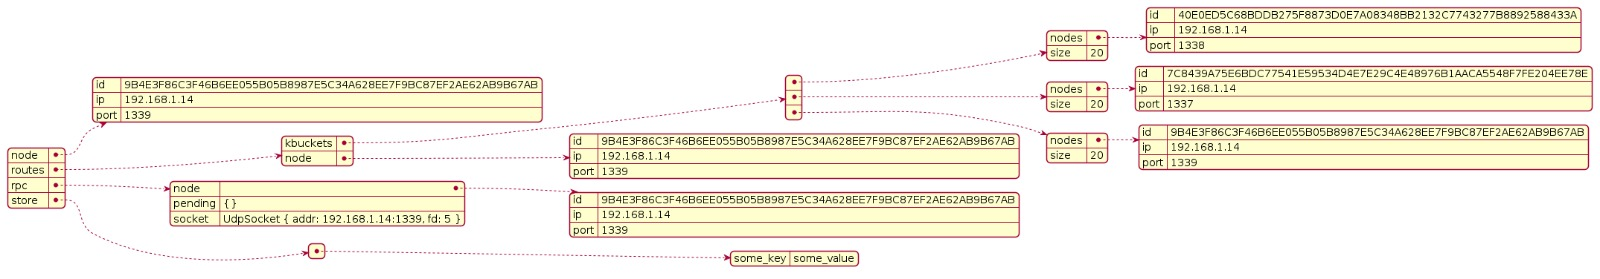
\includegraphics[scale=0.25]{images/kademlia-estrutura.jpeg}
        \caption{Estrutura Kademlia \cite{1}}
        \label{fig:Estrutura Kademlia}
    \end{figure}

%%%falar das 4 funcoes e de como se adiciona um no à rede




    \subsection{Mecanismos de confiança e de comunicação gossip}
    Os mecanismos de confiança são métodos utilizados para avaliar a credibilidade e a confiabilidade dos participantes em um sistema distribuído. Eles permitem que nós (ou usuários) determinem a confiabilidade de outros nós na rede com base em suas interações passadas. Esses mecanismos ajudam a prevenir atividades maliciosas, como ataques de Sybil ou fraudes.
    Neste projeto são utilizados mecanismos de confiança baseados em reputação de nós, onde os nós acumulam uma pontuação de reputação com base em seu comportamento na rede. Além disso, são utilizados mecanismos de detecção de nós mal-intencionados baseados em comportamento suspeito. Esta função que determina a reputação, ou seja o grau de confiança de cada nó está descrita no nosso código como: \textit{node\_find\_bucket\_index\_thrust}.

    Os mecanismos de comunicação gossip são protocolos usados para trocar informações em um sistema distribuído de forma confiável e eficiente. Estes protocolos envolvem a disseminação de informações para um subconjunto aleatório de nós na rede. Os nós então retransmitem as informações para outro subconjunto aleatório de nós, e o processo repete-se até que todos os nós tenham a informação. Isso torna o processo de disseminação de informações mais eficiente, seguro e tolerante a falhas.

    o protocolo gossip utilizado neste trabalho é o protocolo \textit{push-based gossip}, que envolve o envio de mensagens para vizinhos escolhidos aleatoriamente e confiáveis, que por sua vez enviam as mensagens para outros vizinhos confiáveis e assim por diante. Isso ajuda a distribuir informações pela rede de forma eficiente e confiável, sem sobrecarregar nenhum nó específico.

    \subsection{Ataques de Sybil e Eclipse}

    Um ataque eclipse é um tipo de ataque em que um atacante tenta isolar um nó específico em uma rede distribuída, controlando todos os nós vizinhos desse nó. Com isso, o atacante pode controlar a comunicação com o nó isolado, bloqueando ou manipulando informações.

    Para garantir que a rede seja resistente a esse tipo de ataque, o projeto utiliza uma abordagem baseada no protocolo Kademlia DHT, que é resistente a ataques eclipse. Esse protocolo funciona distribuindo os nós na rede usando um sistema de hash de endereços, de modo que cada nó só conhece os vizinhos mais próximos na tabela hash.

    Além disso, o projeto também implementa mecanismos de confiança para garantir que apenas nós confiáveis participem da rede. Esses mecanismos de confiança incluem a reputação do nó, que é baseada em sua taxa de sucesso de transações anteriores, e a \textit{proof-of-work} (PoW), que impõe um custo computacional aos nós que desejam ingressar na rede.

    Dessa forma, a combinação de um protocolo resistente a ataques eclipse com mecanismos de confiança robustos ajuda a garantir que a rede seja segura e resiliente a esse tipo de ataque.

    Um ataque Sybil é um tipo de ataque em que um único indivíduo cria várias identidades falsas na rede para obter um controle desproporcional sobre a rede ou para manipular a opinião pública. Isso pode ser feito para comprometer a integridade da rede, prejudicar sua confiabilidade ou controlar as operações em benefício próprio.

    A rede Kademlia é resistente a ataques Sybil, pois utiliza o algoritmo de roteamento baseado em XOR para localizar nós na rede. Esse algoritmo torna difícil para um atacante Sybil controlar muitos nós, pois cada nó na rede é identificado por um ID único. Além disso, a rede Kademlia utiliza um mecanismo de autenticação baseado em chaves públicas, o que impede que um atacante crie identidades falsas sem acesso às chaves privadas correspondentes.

    Por fim, os mecanismos de confiança ajudam a proteger a rede contra ataques Sybil, já que incluem a avaliação de reputação de nós com base em seu comportamento passado e o uso de um sistema de votação baseado em nós confiáveis para impedir que os nós maliciosos ganhem controle sobre a rede. Combinados, esses mecanismos tornam a rede mais resistente a ataques Sybil.\\

    \section{Registro distribuído e seguro (\textit{Secure Distributed ledger})}
    Baseado em uma abordagem sem permissão
    • Ou seja, pública
    • Os nós não precisam ser conhecidos "a priori"
    • Deve ser modular
    • Suporta PoW como o principal mecanismo de consenso
    • Suporte opcional para:
    • Suporte para Proof-of-Stake como opção
    • Abordagem com permissão baseada em consenso BFT.

    O registro distribuído é implementado utilizando a blockchain como mecanismo de armazenamento. As transações são salvas usando o consenso Proof-of-Work (PoW), que é responsável por validar as transações e adicionar novos blocos à cadeia. A criptografia de chave pública é utilizada para garantir a segurança das transações. O registro distribuído é modular, permitindo a adição de novos mecanismos de consenso, como Proof-of-Stake (PoS) ou BFT.\\


    \section{Mecanismos de leilão (\textit{Auction mechanisms})}

    Capaz de suportar vendedores e compradores
    • Usando um leilão com atributo único
    • Seguindo o modelo de leilão inglês
    • As transações (leilões e lances) devem ser salvas usando o registro
    • Usar criptografia de chave pública
    • Usando um sistema de publicador/assinante para suportar os leilões
    • Construído em cima do Kademlia.

    Os mecanismos de leilão utilizados são baseados no modelo de leilão inglês, utilizando um atributo único para cada leilão. Os leilões são suportados por um sistema de publicador/assinante, permitindo que os participantes da rede possam acompanhar as informações sobre os leilões em tempo real. As transações de leilão e lances são salvas na blockchain, permitindo uma maior transparência e segurança nas transações.\\


    \section{Conclusão}
    A implementação de uma rede Kademlia com blockchain para aplicação de leilões proporciona uma plataforma transparente e segura para leilões. A sobreposição P2P segura e o registro distribuído e modular garantem a eficiência e a segurança da rede, enquanto os mecanismos de leilão baseados no modelo de leilão inglês garantem a transparência e a justiça nas transações. O projeto pode ser expandido para incluir novos mecanismos de consenso e de leilão, tornando-o uma aplicação versátil e escalável para a realização de leilões.\\








    \begin{thebibliography}{1}
        \bibitem{}
    \end{thebibliography}

\end{document}


